\section{Testing the Implementation}

In this chapter the algorithm described in chapter \ref{implement} will be used to calculate the intrinsic matrix \textbf{K}, the distortion coefficients $d$ and the estimated distance $z$. This will be done for each recording with the assumption $d(A, B) = 50cm$. Additionally the size of the 3D metal printer will be estimated.\\

In figure \ref{group_fig:dist_green} one can see the images used, which served as the basis for the pixel coordinates of the boundary points for the respective recording.
\vspace{\baselineskip}

\begin{figure}[H]
    \centering
    \begin{minipage}{\textwidth}
        \begin{subcolumns}[0.4\textwidth]
            \subfloat[250\_cm\_distance.h264 (Cropped)]{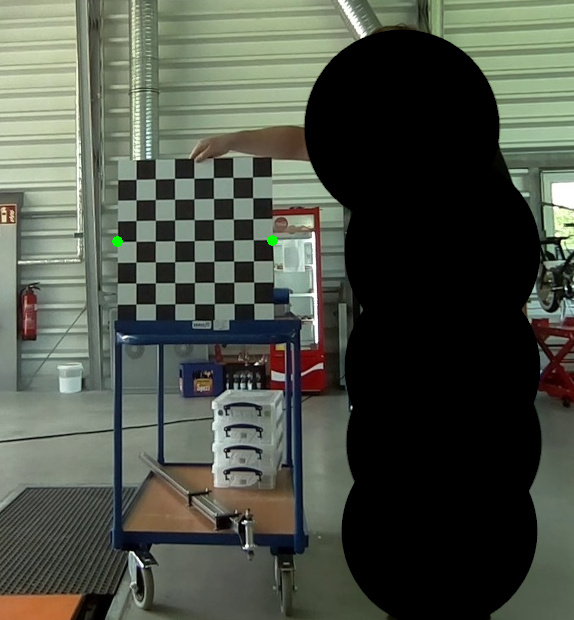
\includegraphics[width=\subcolumnwidth]{image/3/250_undist_cropped_green.jpg}\label{fig:250_dist_green}}
                \nextsubcolumn[0.57\textwidth]
            \subfloat[schwalbe.h264]{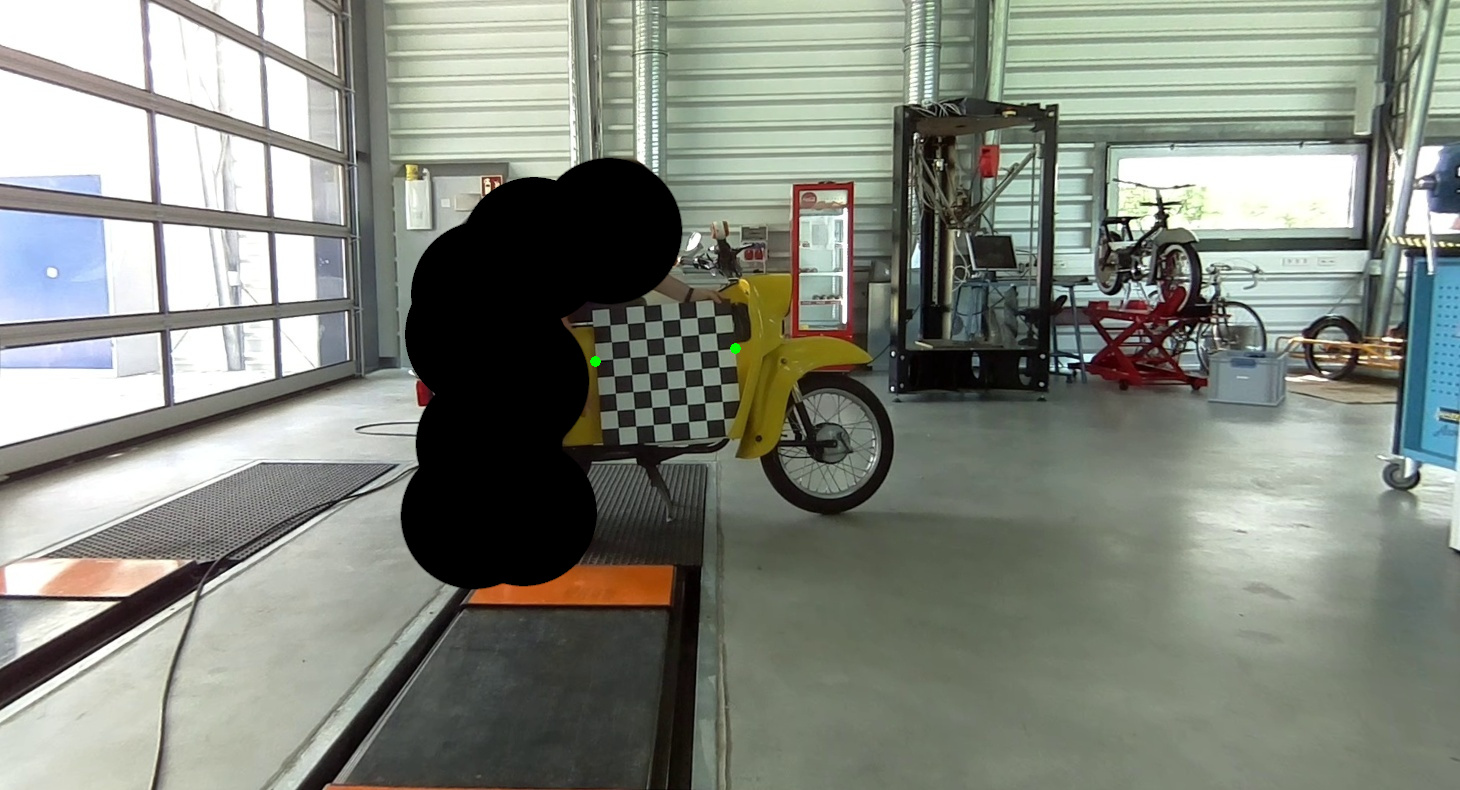
\includegraphics[width=\subcolumnwidth]{image/3/schwalbe_undist_green.jpg}\label{fig:schwalbe_dist_green}}
                \nextsubfigure \vspace{2mm}
            \subfloat[3D\_metal\_printer.h264]{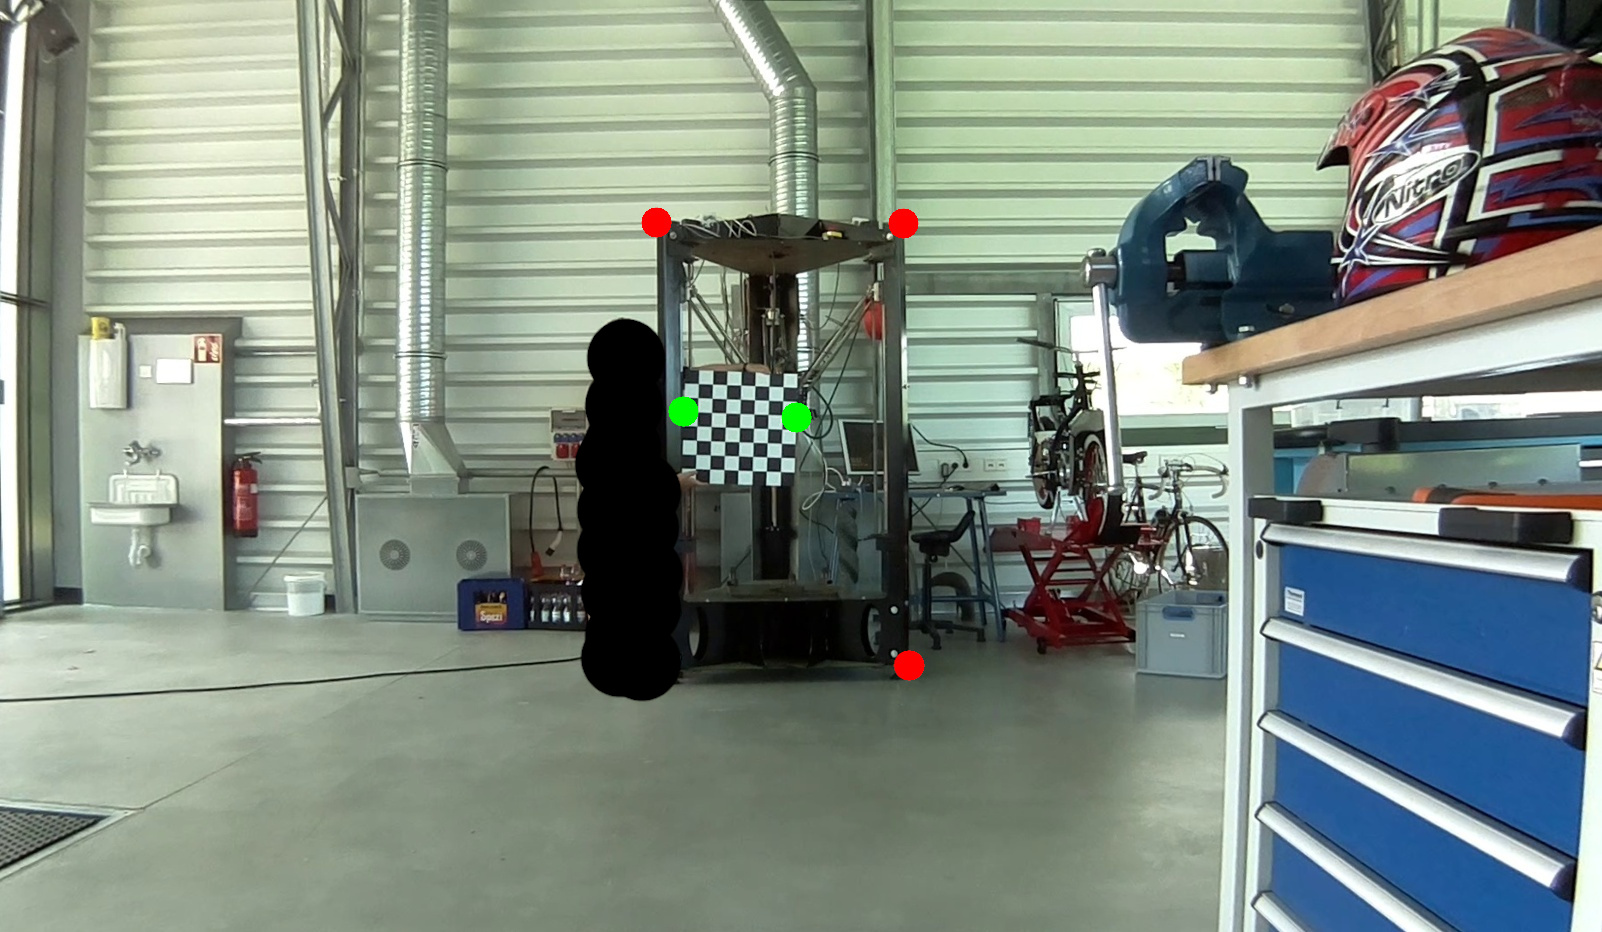
\includegraphics[width=\subcolumnwidth]{image/3/printer_undist_green.jpg}\label{fig:printer_dist_green}}
        \end{subcolumns}
    \end{minipage}
    \caption{Used images for pixel coordinates determination per recording}
    \label{group_fig:dist_green}
\end{figure}

\newpage

\newsubsection{250\_cm\_distance.h264}
The recording \textit{250\_cm\_distance.h264} was run through with the pipelines described in chapter \ref{implement} with a corner size of 6x6. In the process 10 images were used for the calculation of the intrinsic matrix and the distortion coefficients. The intrinsic matrix and the distortion coefficients are as follows:
\vspace{1mm}
\begin{equation*}
    K_1 = 
    \begin{pmatrix}
        1232.4426 & 0 & 827.9823\\
        0 & 1151.2523 & 522.2683\\
        0 & 0 & 1\\
    \end{pmatrix}
\end{equation*}
\vspace{1mm}
\begin{equation*}
    d_1 = (0.03640, -0.79354,  0.06446, -0.09084,  2.27536)
\end{equation*}

The pixel coordinates of the boundary points in figure \ref{fig:250_dist_green} and the calculated estimated distance with equation \ref{eq3} and \ref{eq4} are as follows:

\begin{equation*}
    A = (448,\;391)^{T}\text{;}\; B = (695,\;389)^{T}
\end{equation*}
\begin{align*}
    \Rightarrow \varphi_1 &= \frac{1}{2}\arccos{\frac{\vec{a} \cdot \vec{b}}{|\vec{a}||\vec{b}|}} = \bm{0.19048}\\
    \Rightarrow  z_1 &= \frac{50}{2\tan\varphi}cm = \bm{261.69cm}
\end{align*}
\vspace{-.25\baselineskip}

As a final result we get an estimated distance of $z_1 = 261.69cm$. Since in this recording the object has a known distance of 250cm, the estimated distance is off by 4.67 percent. The deviation can be attributed to the calibration process, where the coefficients of the intrinsic matrix strongly depend on the images and settings used.\\

However, since the deviation from the measured value is less than 10 percent, this result is still acceptable.

\newpage

\newsubsection{schwalbe.h264}
The recording \textit{schwalbe.h264} was run through with the pipelines described in chapter \ref{implement} with a corner size of 6x6. In the process 10 images were used for the calculation of the intrinsic matrix and the distortion coefficients. The intrinsic matrix and the distortion coefficients are as follows:

\vspace{1mm}
\begin{equation*}
    K_2 = 
    \begin{pmatrix}
        1201.3869 & 0 & 824.5984\\
        0 & 1150.7324 & 530.2456\\
        0 & 0 & 1\\
    \end{pmatrix}
\end{equation*}
\vspace{1mm}
\begin{equation*}
    d_2 = (0.03543, -0.80363,  0.08356, -0.07657,  2.25635)
\end{equation*}

The pixel coordinates of the boundary points in figure \ref{fig:schwalbe_dist_green} and the calculated estimated distance with equation \ref{eq3} and \ref{eq4} are as follows:

\vspace{1mm}
\begin{equation*}
    A = (595,\;361)^{T}\text{;}\; B = (735,\;348)^{T}
\end{equation*}
\vspace{-10mm}
\begin{align*}
    \Rightarrow \varphi_2 &= \frac{1}{2}\arccos{\frac{\vec{a} \cdot \vec{b}}{|\vec{a}||\vec{b}|}} = \bm{0.11387}\\
    \Rightarrow  z_2 &= \frac{50}{2\tan\varphi}cm = \bm{438.62cm}
\end{align*}

\vspace{\baselineskip}
\newsubsection{3D\_metal\_printer.h264}
The recording \textit{3D\_metal\_printer.h264} was run through with the pipelines described in chapter \ref{implement} with a corner size of 6x6. In the process 10 images were used for the calculation of the intrinsic matrix and the distortion coefficients. The intrinsic matrix and the distortion coefficients are as follows:

\vspace{1mm}
\begin{equation*}
    K_3 = 
    \begin{pmatrix}
        1251.51 & 0 & 924.7\\
        0 & 1252.07 & 451.81\\
        0 & 0 & 1\\
    \end{pmatrix}
\end{equation*}
\vspace{1mm}
\begin{equation*}
    d_3 = (0.03824, -0.80023,  0.06547, -0.09004,  2.1927)
\end{equation*}

The pixel coordinates of the boundary points in figure \ref{fig:printer_dist_green} and the calculated estimated distance with equation \ref{eq3} and \ref{eq4} are as follows:

\vspace{1mm}
\begin{equation*}
    A = (609,\;384)^{T}\text{;}\; B = (724,\;386)^{T}
\end{equation*}
\vspace{-10mm}
\begin{align*}
    \Rightarrow \varphi_3 &= \frac{1}{2}\arccos{\frac{\vec{a} \cdot \vec{b}}{|\vec{a}||\vec{b}|}} = \bm{0.08797}\\
    \Rightarrow  z_3 &= \frac{50}{2\tan\varphi}cm = \bm{568cm}
\end{align*}

The size of the 3D metal printer was also measured with the pixel coordinates of the boundary points in figure \ref{fig:printer_dist_green} with the equations \ref{eq5}  and \ref{eq6}: 
\vspace{1mm}
\begin{equation*}
    P_1 = (656,\;222)^{T}\text{;}\; P_2 = (903,\;223)^{T}\text{;}\; P_3 = (909,\;665)^{T}
\end{equation*}
\vspace{-10mm}
\begin{align*}
    \Rightarrow width &= \frac{|\bm{P1}-\bm{P2}|}{|\bm{A}-\bm{B}|}\cdot 50cm = \bm{107.38cm}\\
    \Rightarrow  height &= \frac{|\bm{P2}-\bm{P3}|}{|\bm{A}-\bm{B}|}\cdot 50cm = \bm{192.16cm}
\end{align*}

The estimated distance from Schwalbe and 3D metal printer are 4.38m and 5.86m. The size of the 3D metal printer are estimated 1.07x1.92m. Unfortunately, these calculations cannot be checked for accuracy.\\

The height of the 3D metal printer can be checked with another reference in the image: The height of the person holding the checkerboard (which git censored). However, the person in figure \ref{fig:printer_dist_green} is not standing quite straight, which has to be taken into account in the evaluation of the result. The height of the average German male is around 180cm.~\cite{height_person} This turns $d(A, B)$ into $d(A, B) = 180cm$ and we boundary points \textbf{A} and \textbf{B} into $(562,\;359)^{T}$ and $(622,\;689)^{T}$. This gives us a new height of the 3d metal printer of:
\vspace{1mm}
\begin{align*}
    \Rightarrow  height &= \frac{|\bm{P2}-\bm{P3}|}{|\bm{A}-\bm{B}|}\cdot 180cm = \bm{213.89cm}
\end{align*}

With the results 1.92m and 2.13m we can estimate that the 3d metal printer is approximately 2m.
